\section{Background and Objectives}
\begin{figure}
	\centering
	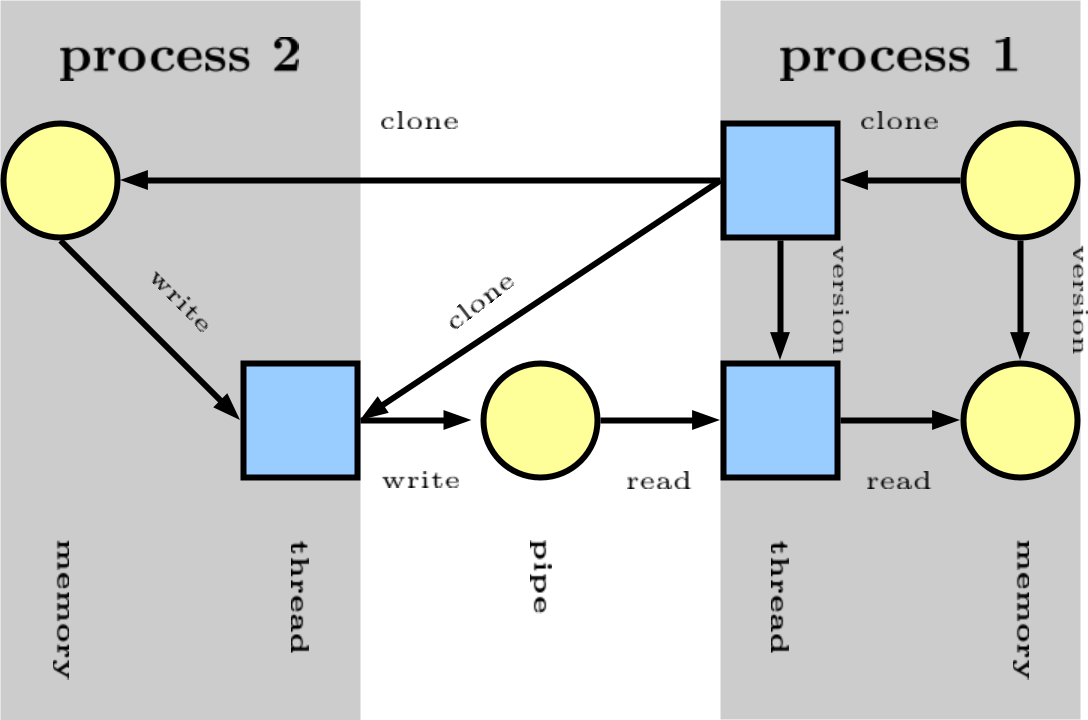
\includegraphics[width=0.7\linewidth]{graph}
	\caption[Provenance graph]{Process 1 clones process 2. Process 2 writes to a pipe. Process 1 read from the same pipe}
	\label{fig:graph}
\end{figure}
\begin{figure}
	\centering
	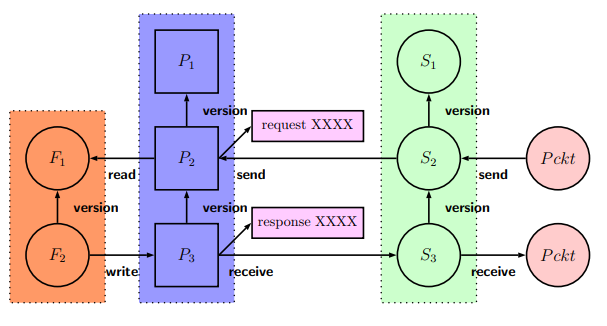
\includegraphics[width=0.7\linewidth]{Annotated-provenance-graph}
	\caption[Provenance graph]{Annotated provenance graph}
	\label{fig:annotated-provenance-graph}
\end{figure}

To provide context for the rest of the paper, we first introduce a few concepts. We introduce the notion of whole-system provenance, provenance graphs, linux security modules and complete mediation property.

\subsection{Whole-system provenance capture}
\label{A little about the graphs}
Data provenance was originally introduced to understand the origin of data in a database. (17,18) According to the W3C (19) standards provenance is defined as a directed acyclic graph (DAG). The vertices in the DAG represent entities(data), activities(transformations of data) and agents(persons or organizations). The edges represent the relationships between these elements. Mapping the graph definition to our system, which is the OS level entities are kernel objects, such as messages, network packets, files etc., but also xattributes, inode attributes, exec call parameters, network addresses, etc.
Activities are the tasks or processes carrying out manipulations on entities causing data flows. The agents are the persons or the organizations, who control the activities on different entities. These are the users and the groups at the OS level. 
 the agents are users and groups. Fig 1 illustrates these concepts. In the example in Fig 1, process 1 clones process 2. Process 2 writes to a pipe and finally process 1 read from the same pipe.
\vskip 0.2in 
Processes exchange information via system calls. Some system calls represent information exchange at some discrete point in time e.g, read, write; others may create shared states, e.g, nmap.


\label{A small recap into data provenance and whole system provenance capture}

There have been multiple whole system provenance capture systems proposed in the past such as HiFi, PASS. However, they had a couple of problems: 1) struggled to keep abreast with current OS releases 2) Did not have whole system provenance capture guarantees 3) generated too much data 4)imposed too much overhead. Learning from the lessons from the past the whole system provenance capture systems, Camflow was introduced which promised to resolve all the above mentioned issues. Camflow addressed the above mentioned shortcomings 1) by leveraging the latest kernel defining to achieve efficiency 2) using a self-contained, easily maintainable implementation relying on Linux Security Modules, Net-filter, and other existing kernel facilities.


\subsection{Linux Security Modules}
\label{LSMs}
Since the kernel version 2.6, Linux added support for a framework to implement security extensions for the kernel called Linux Kernel Modules(LSM)(14). This framework provides a set of hooks strategically
placed in the kernel code associated with felds in internal data
structures for exclusive use by security extensions. The hooks are
functions which can be used by security extensions to (1), allocate,
free, and maintain the security state of various internal data structures having a dedicated security field, and (2), implement security
checks at specific points of execution, based on the security state
and a policy.  Security modules have a chance to apply security
restrictions anywhere a hook is present, but only at these places.
LSM’s original design is the access control and this has dictated the
placement of hooks in the code. . It is thus necessary to verify the
correctness of this placement for the purpose of information flow
tracking to ensure that information flow trackers. 
\vskip 0.2in
Since, Camflow uses LSMs and Net-Filters to capture the system provenance, the need to verify the correct placement of hooks for Camflow becomes necessary. 



\subsection{Complete Mediation Property}
The first goal of our contribution is to verify the property called "Complete Mediation property". According to this property for any execution path in the kernel starting with a system call and leading to an information flow, there is at least one LSM hook in the path which is reached before the flow is performed. It's important to verify this property. The reason is because if there exists a path generating a flow but not going through any LSM hooks, then there exists an opening for a malicious program to perform illegal actions without triggering any alarms. This is because information flow monitor can only react when one of the hooks is reached. 
\vskip 0.1in
In order to identify all the paths which lead to information flows requires solving two common problems in static analysis. The first problem is that the number of execution paths is infinite because of loops and recursions in the code. In order to finitize the code a subset is selected which should be sufficient to draw a conclusion for all the paths. In other words constructing an abstraction of the code which can be mapped to the concrete code after the analysis is required. The second problem  is that many execution paths that appear in the control flow graph (CFG) cannot actually be taken. These are called as the infeasible paths(20).  
\vskip 0.2in
For our analysis we consider all the system calls in the kernel version 4.20. Flow control requires knowing precisely when an information flow starts and when it stops. If this information is not available, it is not possible to maintain a correct representation of all flows currently taking place in the system at any given time. Since LSM was designed with access control in mind, some hooks might be missing to perform information flow tracking in every kernel update that comes. However, using static analysis we can find if some hooks are missing to perform information flow tracking. 
%\textbf{Georget et al methodology}


\label{Information flow}
The purpose of information flow control is to monitor the way in which information is disseminated in the system once it is out of its original container. This is unlike access control which can only enforce rules on how whose containers are accessed. Several scientific and technical challenges exist in ensuring complete information flow. One of them being the large Linux kernel code base. Georget tackles this issue in his work.



%\label{Georget methodology}
%In order to improve the state of art of the information flow systems, Georget et. al developed a  plugin for the GCC compiler to easily extract and visualize control flow graphs of kernel functions...


\label{Camflow}
Camflow which utilizes LSM for the whole-system provenance capture. It collects the provenance data and constructs provenance graphs from the collected data. Now that we are aware that Georget's methodology ensures the placement of hooks such that complete information flow is possible, we prove/disprove that the violations are reflected in the provenance graphs.

